\documentclass[oneside,a4paper,14pt]{extarticle}
\usepackage[a4paper,letterpaper,top=20mm,bottom=20mm,left=20mm,right=10mm]{geometry}
\usepackage[russian]{babel}
\usepackage{indentfirst}
\usepackage{graphicx}
\usepackage{caption}
\usepackage{titlesec}
\usepackage{minted, fancyvrb}
\usepackage{hyperref}
\usepackage{enumitem}

% Форматирование листингов с кодом
\setminted{style = rainbow_dash, fontsize = \small} % https://pygments.org/styles/

% Форматирование заголовков
\titleformat{\section}{\normalsize\bfseries}{\thesection}{1em}{}
\titleformat{\subsection}{\normalsize\bfseries}{\thesubsection}{1em}{}
\titleformat{\subsubsection}{\normalsize\bfseries}{\thesubsubsection}{1em}{}

% Интерлиньяж и абзац
\renewcommand\baselinestretch{1.33}

\setlength{\parindent}{1.25cm}  % длина красной строки

% Для всех списков
\setlist[enumerate]{
  left=0.5\parindent,       % отступ слева
  label=\arabic*.,       % цифры
  itemsep=0pt,           % расстояние между пунктами
  topsep=5pt,            % отступ сверху
  partopsep=0pt,         % дополнительный отступ сверху, если абзац до списка
  parsep=0pt             % отступ между абзацами внутри пункта
}

\setlist[itemize]{
  left=0.5\parindent,       % отступ слева
  itemsep=0pt,           % расстояние между пунктами
  topsep=5pt,            % отступ сверху
  partopsep=0pt,
  parsep=0pt
}

% Гиперссылки
\hypersetup{
  colorlinks=true,
  linkcolor=black,
  urlcolor=blue,
  pdfborder={0 0 0},
  pdftitle={Бот для игры "Морской Бой"},
  pdfauthor={Черкасов А.А.}
}

\begin{document}

\newpage
\thispagestyle{empty}
\begin{center}
  МИНИСТЕРСТВО НАУКИ И ВЫСШЕГО ОБРАЗОВАНИЯ РОССИЙСКОЙ ФЕДЕРАЦИИ ФЕДЕРАЛЬНОЕ ГОСУДАРСТВЕННОЕ БЮДЖЕТНОЕ УЧРЕЖДЕНИЕ ВЫСШЕГО ОБРАЗОВАНИЯ\\
  <<ВЯТСКИЙ ГОСУДАРСТВЕННЫЙ УНИВЕРСИТЕТ>>\\
  Институт математики и информационных систем\\
  Факультет автоматики и вычислительной техники\\
  Кафедра электронных вычислительных машин
\end{center}
\vspace{10mm}

\hfill
\begin{tabular}{l}
  \footnotesize Дата сдачи на проверку:                                          \\
  \footnotesize <<\rule[-1mm]{5mm}{0.10mm}\/>>\rule[-1mm]{20mm}{0.10mm}\ 2025 г. \\
  \footnotesize Проверено:                                                       \\
  \footnotesize <<\rule[-1mm]{5mm}{0.10mm}\/>>\rule[-1mm]{20mm}{0.10mm}\ 2025 г. \\
\end{tabular}
\vfill

\begin{center}
  Отчёт по лабораторной работе №3\\
  по дисциплине\\
  <<Теория Автоматов>>\\
\end{center}
\vspace{25mm}
\noindent
\begin{tabular}{ll}
  Разработал студент гр. ИВТб-2301-05-00 & \hspace{18mm}\rule[-1mm]{30mm}{0.10mm}\,/Черкасов А. А./ \\
                                         & \hspace{25.5mm}\footnotesize(подпись)                    \\
  Старший Преподователь                  & \hspace{18mm}\rule[-1mm]{30mm}{0.10mm}\,/Мельцов В. Ю./  \\
                                         & \hspace{25.5mm}\footnotesize(подпись)                    \\
\end{tabular}

\noindent
\begin{tabular}{lp{58mm}r}
  Работа защищена &  & \hspace{13mm}<<\rule[-1mm]{5mm}{0.10mm}\/>>\rule[-1mm]{30mm}{0.10mm}\ 2025 г.
\end{tabular}
\vfill

\begin{center}
  Киров\\
  2025
\end{center}

\newpage\thispagestyle{plain}

\section*{Цель лабораторной работы}
Разработка бота для игры "Морской Бой" со стратегиями поиска и добивания кораблей противника.

\section*{Задание}
Разработать бота для игры "Морской Бой", который:
\begin{enumerate}
  \item Реализует эффективные стратегии поиска кораблей в зависимости от их размера
  \item Автоматически переключается в режим добивания при попадании
  \item Определяет направление корабля и завершает его уничтожение
  \item Ведет учет состояния поля противника и счетчиков живых кораблей
\end{enumerate}

\section*{Реализация бота}

Бот реализован на языке Pascal и состоит из следующих основных компонентов:

\begin{itemize}
  \item[$-$] \texttt{makeShot()} $-$ основная функция выбора клетки для выстрела
  \item[$-$] \texttt{processResult()} $-$ функция обработки результата выстрела
  \item[$-$] \texttt{searchMode()} $-$ функция выбора клетки в режиме поиска
  \item[$-$] \texttt{finishingMode()} $-$ функция добивания корабля
\end{itemize}

\subsection*{Игровые элементы}

Игра "Морской Бой" ведется на поле 10×10 клеток с координатами от (0,0) до (9,9).

\textbf{Флот состоит из:}
\begin{itemize}
  \item[$-$] 1 четырехпалубного корабля
  \item[$-$] 2 трехпалубных кораблей
  \item[$-$] 3 двухпалубных кораблей
  \item[$-$] 4 однопалубных кораблей
\end{itemize}

\textbf{Результаты выстрелов:}
\begin{itemize}
  \item[$-$] 0: Промах
  \item[$-$] 2: Попадание (корабль не уничтожен)
  \item[$-$] 3: Уничтожение (корабль полностью уничтожен)
\end{itemize}

\textbf{Состояния клеток поля противника:}
\begin{itemize}
  \item[$-$] 0: Неизвестная (не стреляли)
  \item[$-$] 1: Промах
  \item[$-$] 2: Попадание
  \item[$-$] 3: Уничтоженный корабль
  \item[$-$] 4: Невозможная (вокруг уничтоженного корабля)
\end{itemize}

\subsection*{Внутренние состояния бота}

Бот поддерживает следующие внутренние состояния:

\begin{itemize}
  \item[$-$] Режимы работы: поиск 4п, поиск 3п, поиск оставшихся или добивание
  \item[$-$] Матрица поля противника 10×10
  \item[$-$] Счетчики живых кораблей по размерам (4,3,2,1 палуб)
  \item[$-$] Очередь клеток для стрельбы в режиме поиска
  \item[$-$] Список попаданий в текущий корабль
  \item[$-$] Направление корабля: горизонтальное/вертикальное
\end{itemize}

\subsection*{Основной цикл работы}

\subsubsection*{Инициализация игры}

При начале новой игры бот:
\begin{enumerate}
  \item Устанавливает начальный индекс расстановки
  \item Инициализирует поле противника всеми нулями
  \item Устанавливает счетчики кораблей: 4-3-2-1
  \item Переходит в режим поиска четырехпалубных кораблей
  \item Инициализирует очередь поиска
\end{enumerate}

\subsubsection*{Выбор выстрела}

В зависимости от текущего режима:
\begin{itemize}
  \item[$-$] \textbf{Режим поиска}: Выбирает клетку из оптимизированной очереди
  \item[$-$] \textbf{Режим добивания}: Рассчитывает следующий выстрел для завершения корабля
\end{itemize}

\subsubsection*{Обработка результата}

После каждого выстрела бот анализирует результат:
\begin{itemize}
  \item[$-$] \textbf{Промах (0)}: Клетка помечается как 1
  \item[$-$] \textbf{Попадание (2)}: Клетка помечается как 2, добавляется в список попаданий, активируется режим добивания
  \item[$-$] \textbf{Уничтожение (3)}: Клетки корабля помечаются как 3, вокруг них - как 4, уменьшается счетчик типа корабля, сброс в режим поиска
\end{itemize}

\subsection*{Режим поиска}

Стрельба ведется по оптимизированной стратегии, зависящей от размера самого большого живого корабля.

\subsubsection*{Поиск четырехпалубных (6 проходов)}

\begin{enumerate}
  \item Проход 1 смещение(0,0): (0,0), (0,4), (0,8), (4,0), (4,4), (4,8), (8,0), (8,4), (8,8)
  \item Проход 2 смещение(1,1): (1,1), (1,5), (1,9), (5,1), (5,5), (5,9), (9,1), (9,5), (9,9)
  \item Проход 3 смещение(2,2): (2,2), (2,6), (6,2), (6,6)
  \item Проход 4 смещение(3,3): (3,3), (3,7), (7,3), (7,7)
  \item Проход 5 смещение(4,4): (4,4), (4,8), (8,4), (8,8)
  \item Проход 6 смещение(5,5): (5,5), (5,9), (9,5), (9,9)
\end{enumerate}

\subsubsection*{Поиск трехпалубных (4 прохода)}

\begin{enumerate}
  \item Проход 1 смещение(0,0): (0,0), (0,3), (0,6), (0,9), (3,0), (3,3), (3,6), (3,9), (6,0), (6,3), (6,6), (6,9), (9,0), (9,3), (9,6), (9,9)
  \item Проход 2 смещение(1,1): (1,1), (1,4), (1,7), (4,1), (4,4), (4,7), (7,1), (7,4), (7,7)
  \item Проход 3 смещение(2,2): (2,2), (2,5), (2,8), (5,2), (5,5), (5,8), (8,2), (8,5), (8,8)
  \item Проход 4 смещение(3,3): (3,3), (3,6), (3,9), (6,3), (6,6), (6,9), (9,3), (9,6), (9,9)
\end{enumerate}

\subsubsection*{Поиск двухпалубных и однопалубных}

Очередь заполняется всеми неизвестными клетками слева направо, сверху вниз.

\subsection*{Режим добивания}

Активируется при первом попадании в корабль (результат = 2).

\subsubsection*{Одиночное попадание}

Стрельба ведется в 4 направления от клетки попадания: вверх, вниз, влево, вправо.

\subsubsection*{Два и более попадания}

Определение направления корабля:
\begin{itemize}
  \item[$-$] Если все попадания в одном ряду → горизонтальное направление
  \item[$-$] Если все попадания в одном столбце → вертикальное направление
\end{itemize}

\subsubsection*{Добивание горизонтального корабля}

\begin{enumerate}
  \item Сортировка попаданий по столбцу (координате X)
  \item Стрельба вдоль линии корабля (заполнение пробелов между попаданиями)
  \item Стрельба на одну клетку за крайними попаданиями (влево и вправо)
\end{enumerate}

\subsubsection*{Добивание вертикального корабля}

Аналогично, но сортировка по строке (координате Y), стрельба вверх и вниз.

\subsubsection*{При уничтожении корабля}

\begin{enumerate}
  \item Клетки попаданий помечаются как 3 (уничтоженный корабль)
  \item Вокруг корабля все соседние клетки помечаются как 4 (невозможные)
  \item Уменьшается счетчик типа корабля
  \item Сбрасывается режим в поиск
\end{enumerate}

\subsection*{Практические примеры}

\subsubsection*{Пример 1: Поиск и добивание четырехпалубного корабля}

Противник разместил четырехпалубный корабль горизонтально на клетках (2,3), (2,4), (2,5), (2,6).

{\footnotesize
\begin{tabular}{|c|c|p{4cm}|c|c|}
  \hline
  Выстрел & Результат & Действия бота & Следующий выстрел & Примечание \\
  \hline
  (0,0) & 0 & Промах, клетка → 1 & (0,4) & Поиск 4п, проход 1 \\
  (0,4) & 0 & Промах, клетка → 1 & (2,2) & Продолжение поиска \\
  (2,2) & 2 & Попадание, клетка → 2, список попаданий = [(2,2)], режим добивания & (1,2) & Первое попадание \\
  (1,2) & 0 & Промах, клетка → 1 & (2,1) & Проверка вверх \\
  (2,1) & 0 & Промах, клетка → 1 & (2,3) & Проверка влево \\
  (2,3) & 2 & Попадание, клетка → 2, список = [(2,2),(2,3)], направление горизонтальное & (2,4) & Второе попадание \\
  (2,4) & 2 & Попадание, клетка → 2, список = [(2,2),(2,3),(2,4)] & (2,5) & Продолжение линии \\
  (2,5) & 2 & Попадание, клетка → 2, список = [(2,2),(2,3),(2,4),(2,5)] & (2,6) & Продолжение линии \\
  (2,6) & 3 & Уничтожение, клетки (2,2)-(2,6) → 3, вокруг → 4, счетчик 4п уменьшен, режим поиска 3п & (0,3) & Корабль уничтожен \\
  \hline
\end{tabular}
}

\subsubsection*{Пример 2: Добивание с определением направления}

Противник имеет трехпалубный корабль вертикально на (4,7), (5,7), (6,7).

{\footnotesize
\begin{tabular}{|c|c|p{4cm}|c|c|}
  \hline
  Выстрел & Результат & Действия бота & Следующий выстрел & Примечание \\
  \hline
  (4,7) & 2 & Попадание, список = [(4,7)], режим добивания & (3,7) & Первое попадание \\
  (3,7) & 0 & Промах, клетка → 1 & (4,6) & Проверка влево \\
  (4,6) & 0 & Промах, клетка → 1 & (4,8) & Проверка вправо \\
  (4,8) & 0 & Промах, клетка → 1 & (5,7) & Проверка вниз \\
  (5,7) & 2 & Попадание, список = [(4,7),(5,7)], направление вертикальное & (6,7) & Второе попадание \\
  (6,7) & 3 & Уничтожение, клетки (4,7)-(6,7) → 3, вокруг → 4, счетчик 3п уменьшен, режим поиска & (0,6) & Корабль уничтожен \\
  \hline
\end{tabular}
}

\newpage

\subsection*{Схема алгоритма}

\begin{figure}[H]
  \centering
  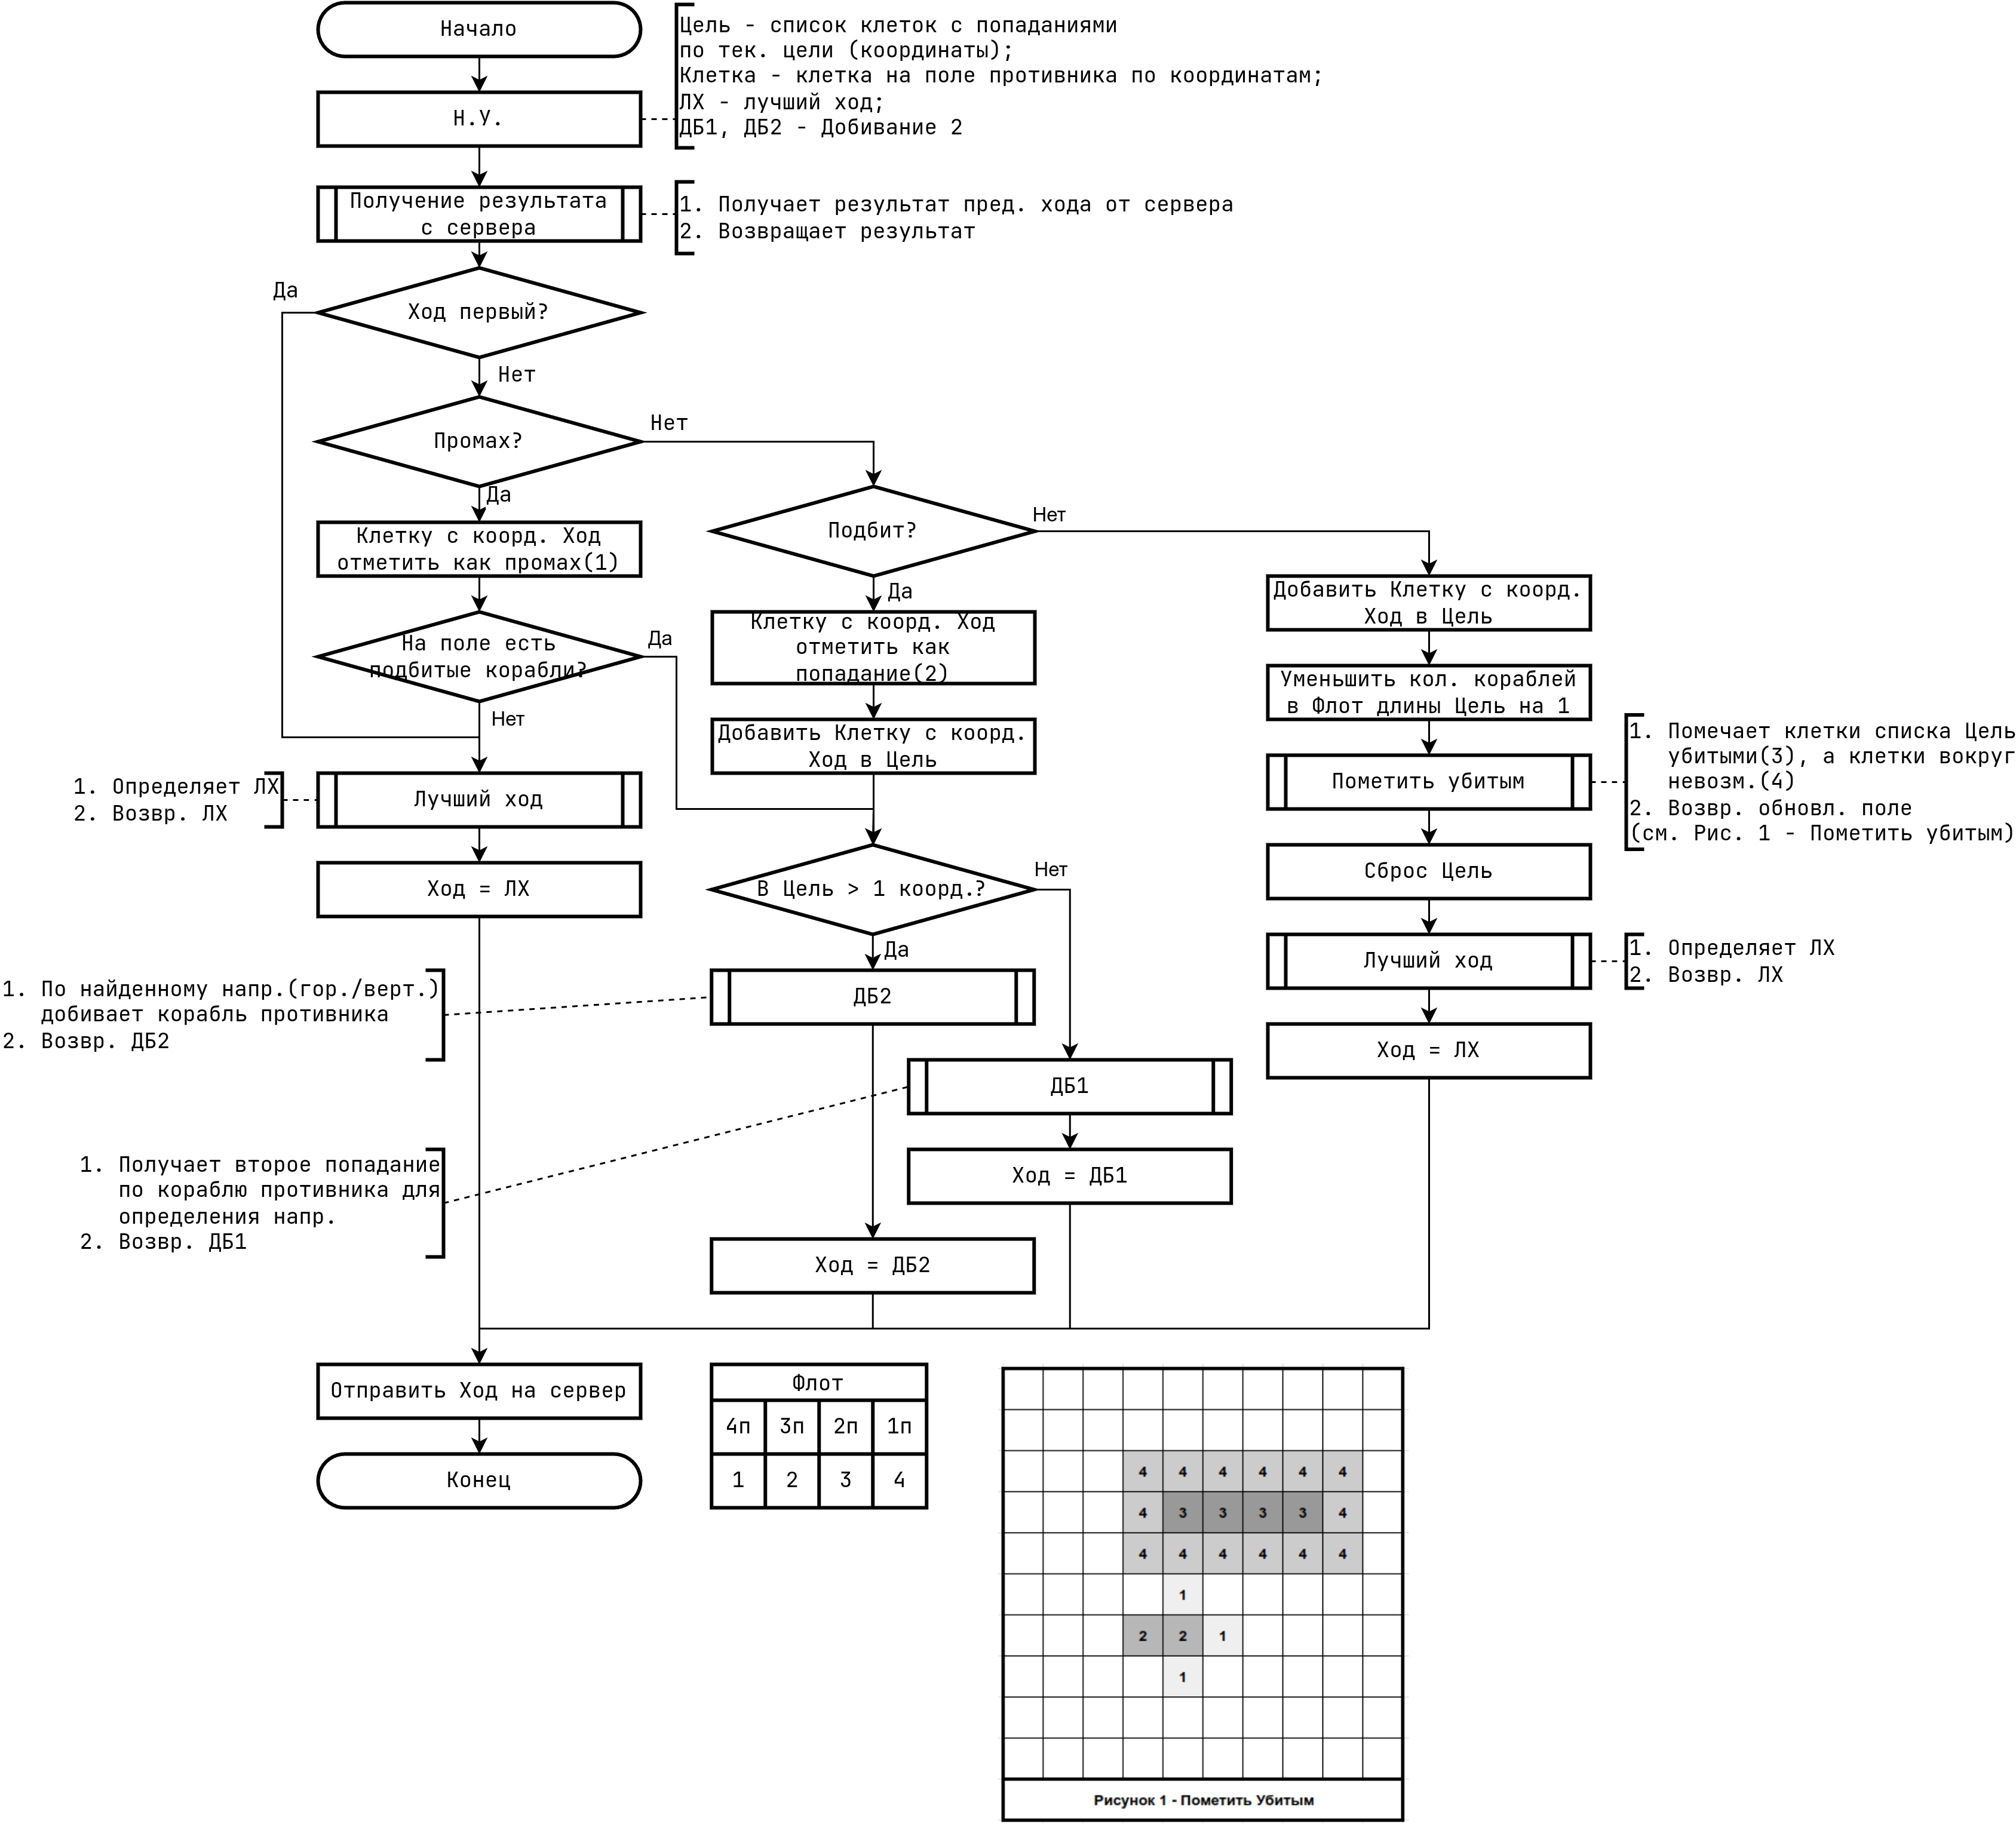
\includegraphics[width=0.9\textwidth]{pics/flowchart_main.png}
  \caption*{Рисунок 1 - Основной алгоритм работы бота}
\end{figure}

\begin{figure}[H]
  \centering
  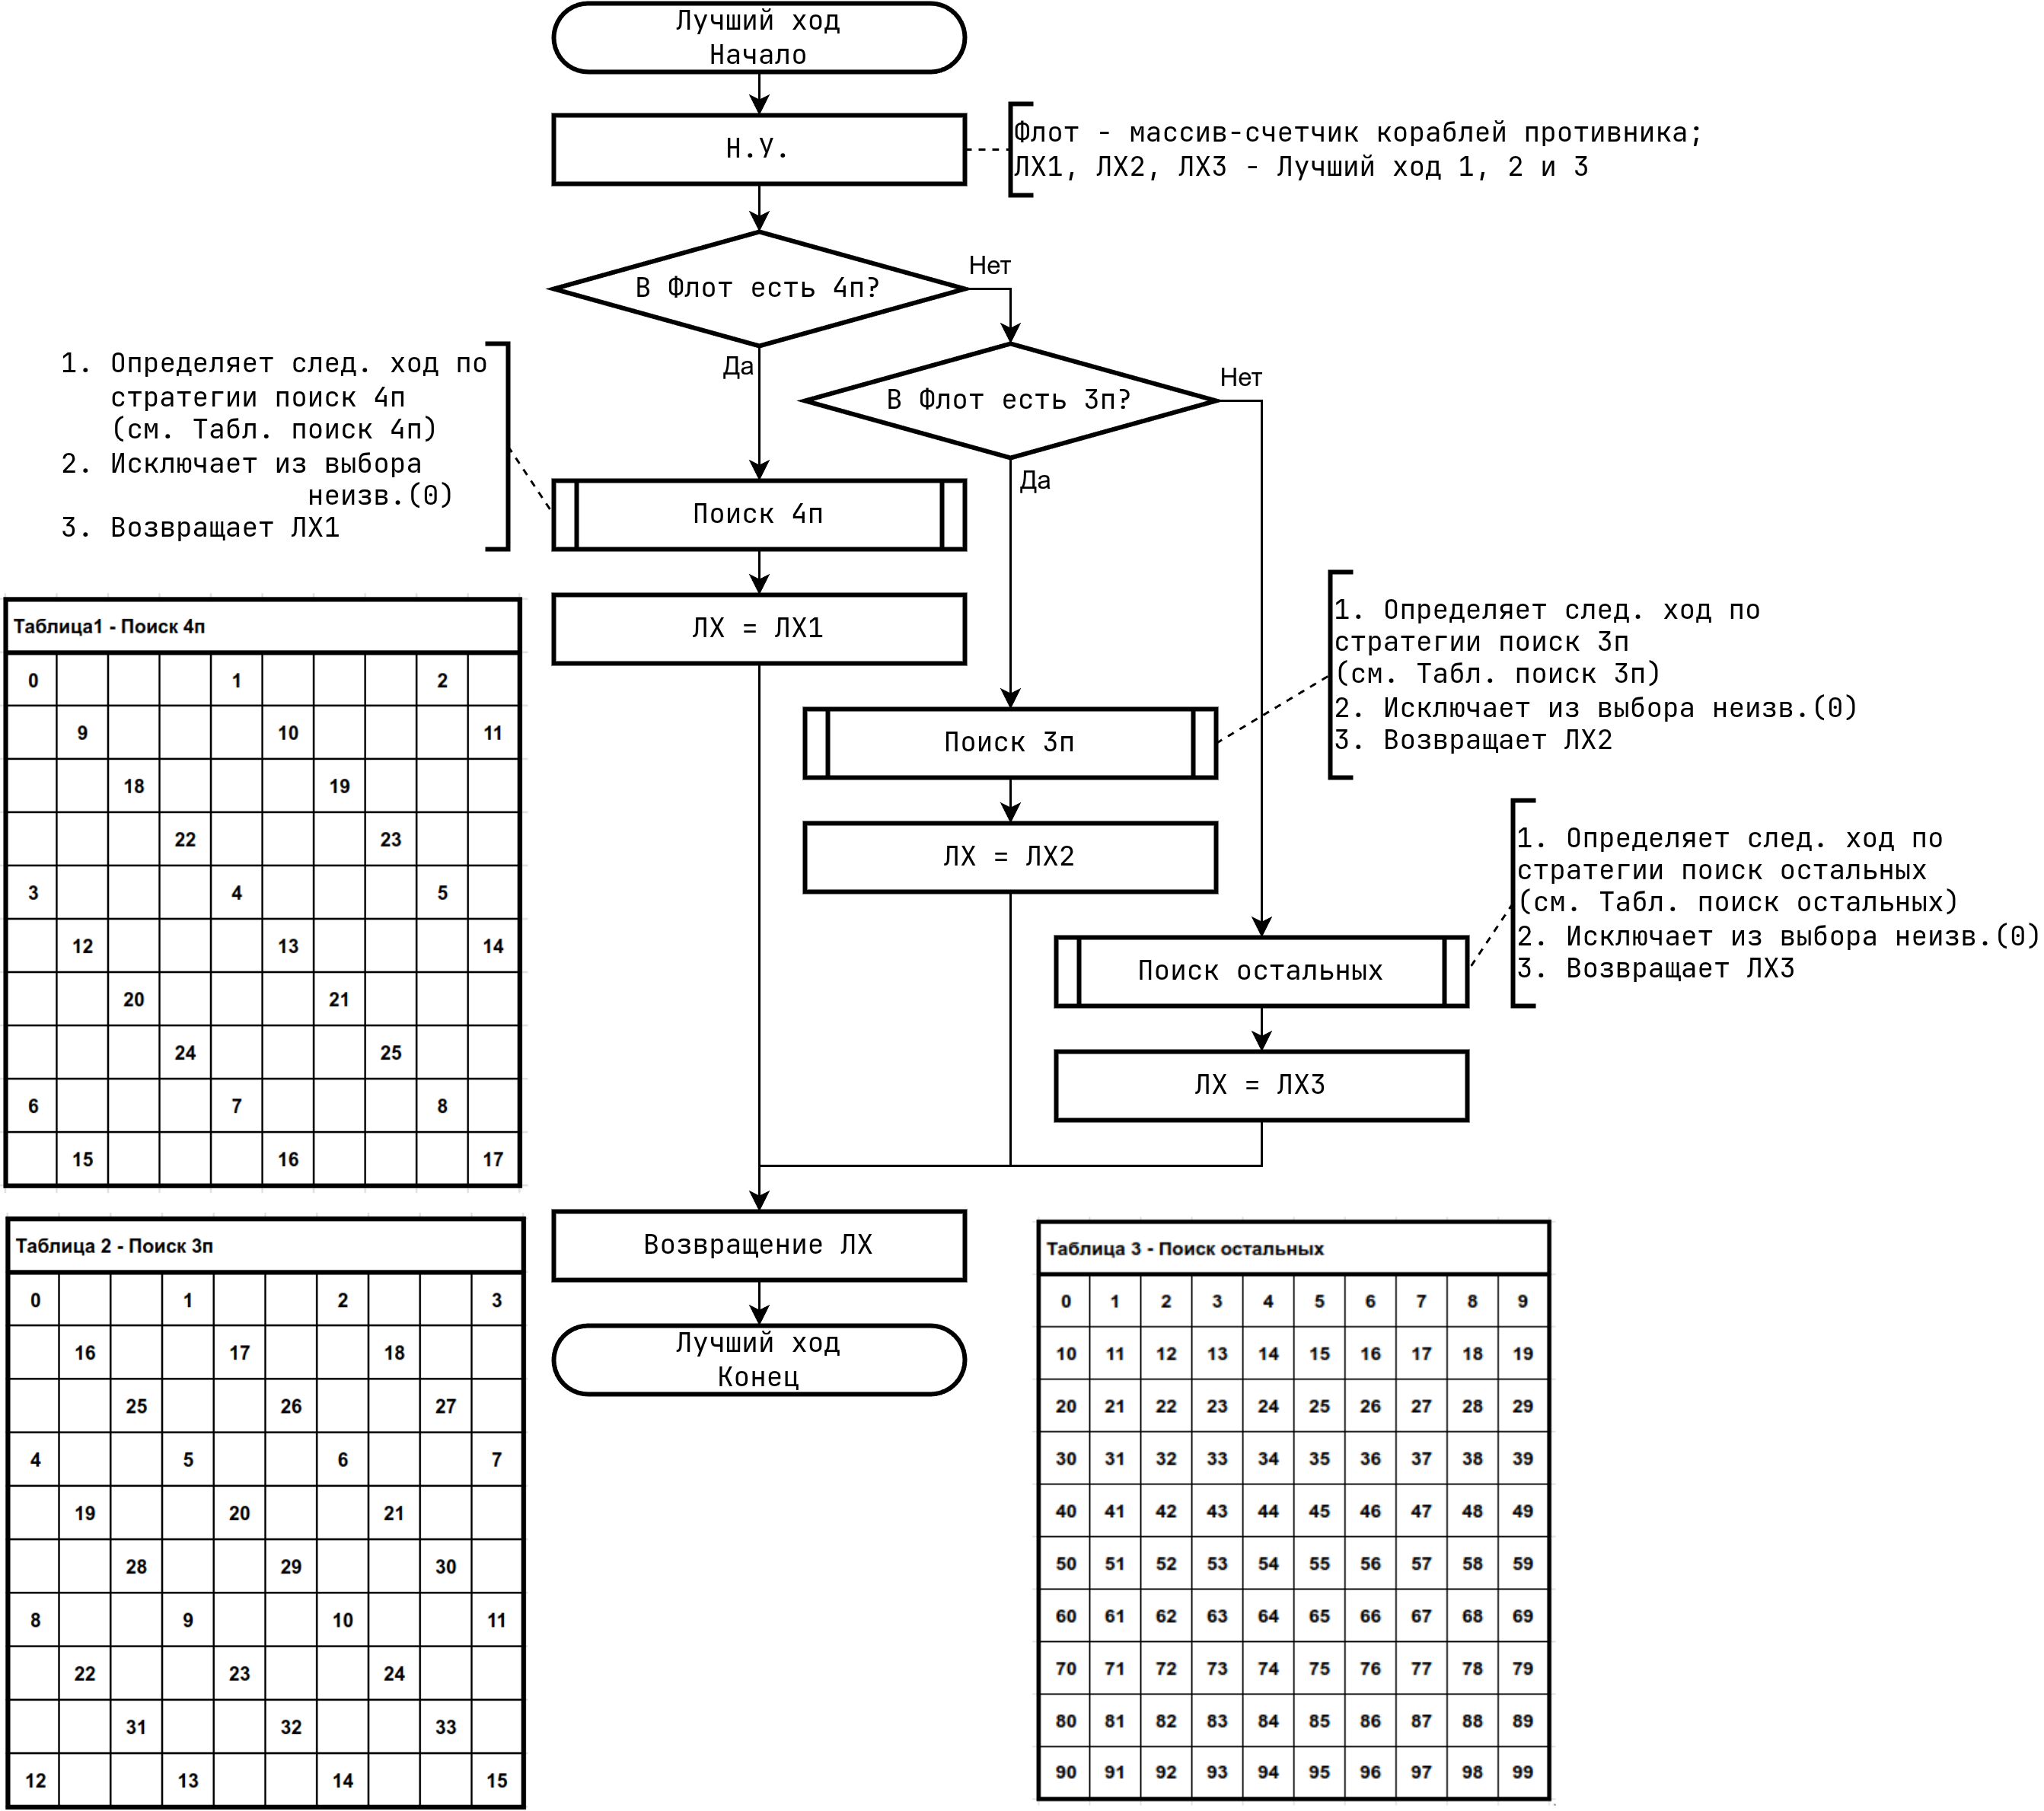
\includegraphics[width=0.9\textwidth]{pics/flowchart_best.png}
  \caption*{Рисунок 2 - Алгоритм выбора клетки в режиме поиска}
\end{figure}

\begin{figure}[H]
  \centering
  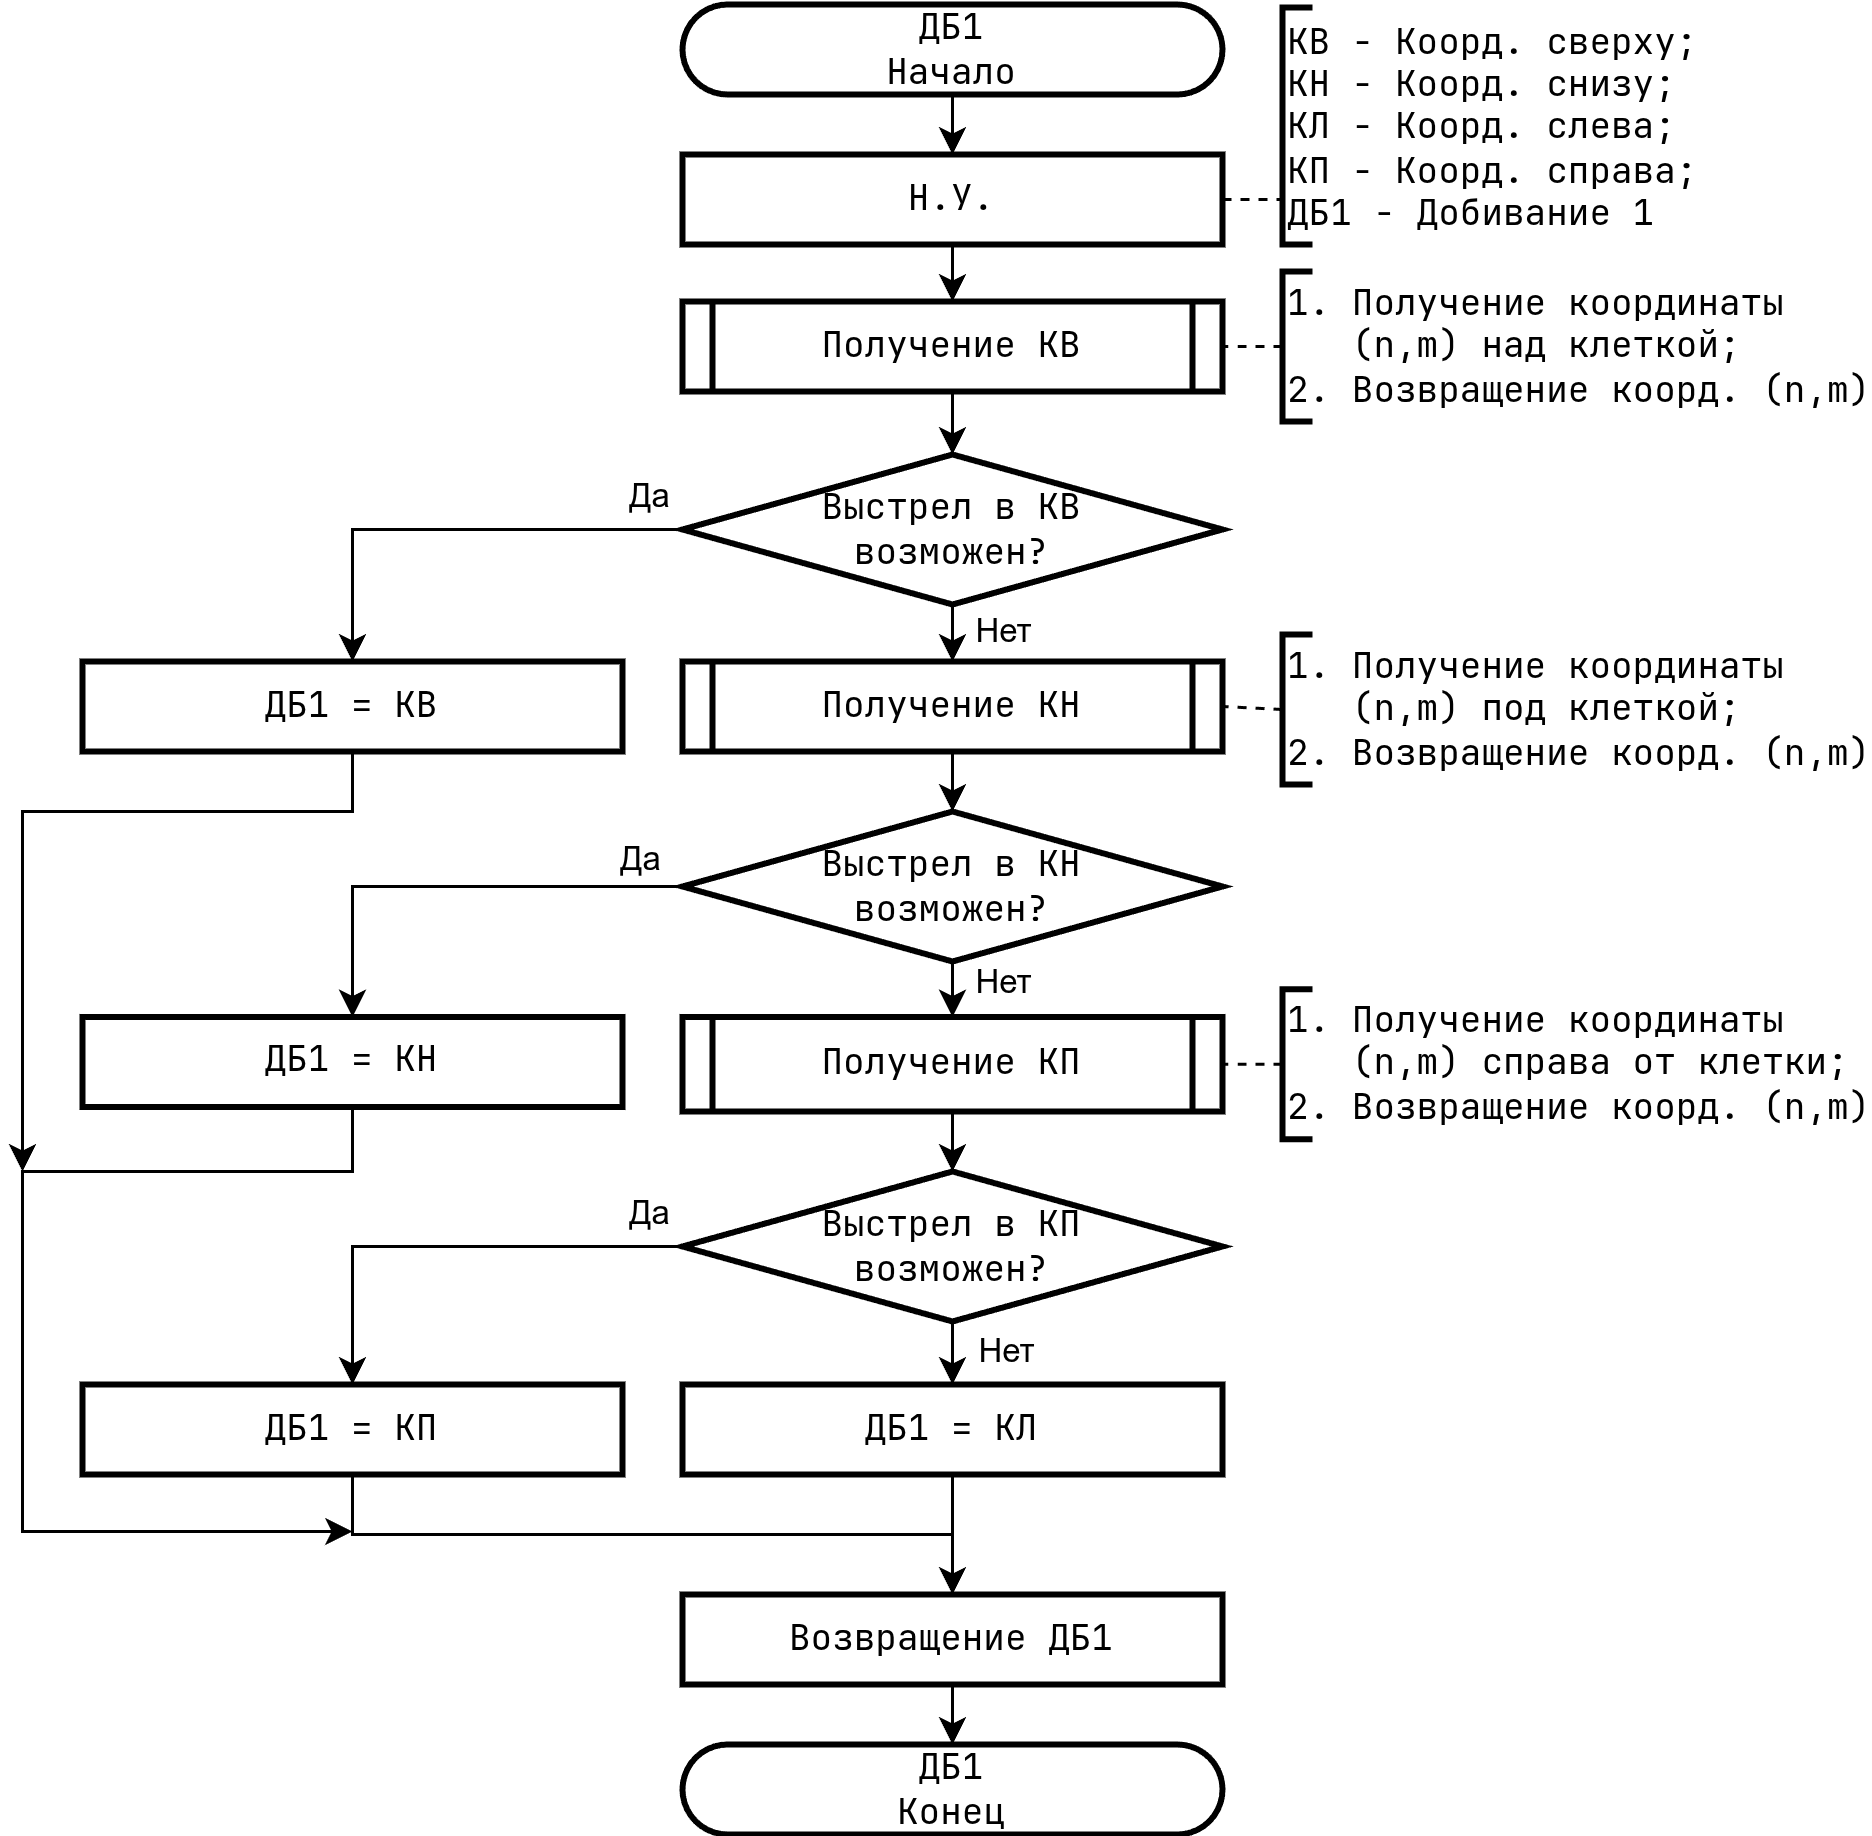
\includegraphics[width=0.9\textwidth]{pics/flowchart_dob.png}
  \caption*{Рисунок 3 - Алгоритм режима добивания (начало)}
\end{figure}

\begin{figure}[H]
  \centering
  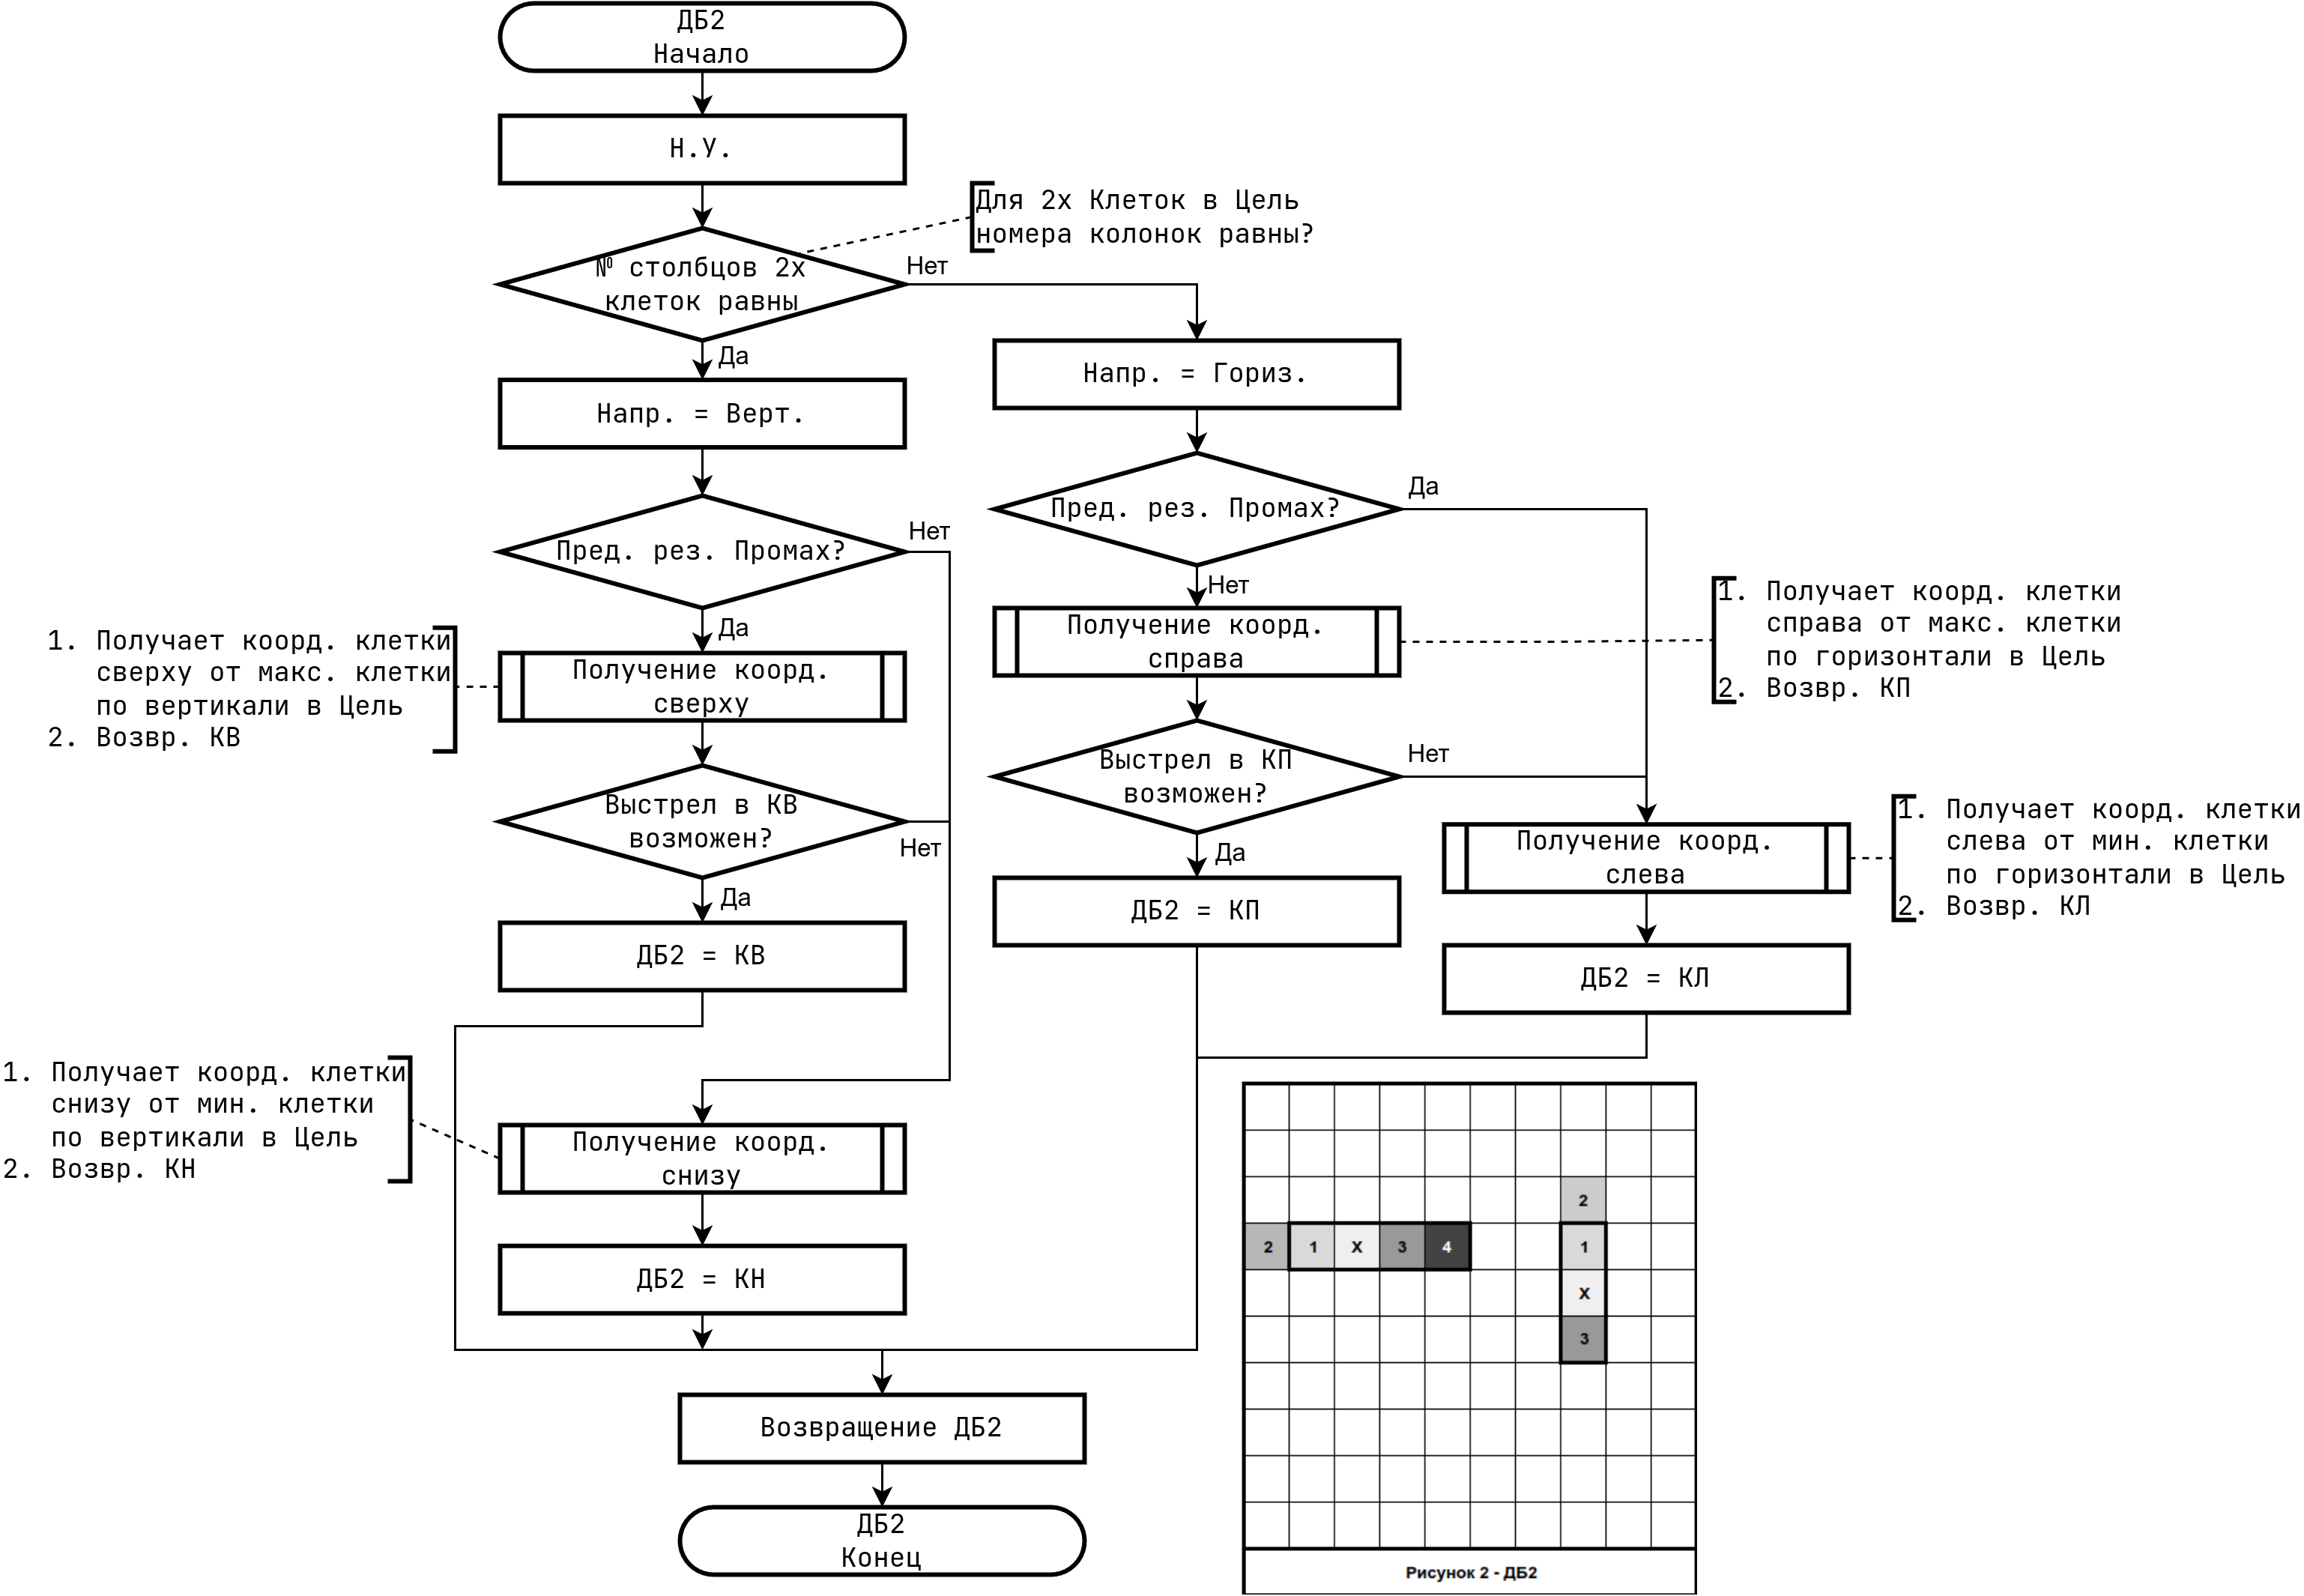
\includegraphics[width=0.9\textwidth]{pics/flowchart_dob_fin.png}
  \caption*{Рисунок 4 - Алгоритм режима добивания (завершение)}
\end{figure}

\newpage

\section*{Вывод}

В ходе выполнения лабораторной работы №3 был разработан бот для игры "Морской Бой" со стратегиями поиска и добивания кораблей. Бот реализует алгоритмы поиска кораблей разных размеров, автоматическое переключение в режим добивания при попадании, определение направления корабля и ведение состояния поля противника. Бот написан на языке Pascal.

\end{document}
